% Open Orders report macro v2.8: one build, from the exports to the workbook.
% Alternate of open-orders-macro-flow.tex: station 1 shows two exports and no open question; otherwise the same page.
% One 11 x 17 landscape page (ledger, 17 x 11 in) drawn in TikZ, read top left to bottom right: title and what the macro does for every MSA,
% stations 1 to 5 with the setup-check gate and the UNMAPPED loop, the title block.
% Statements come from output/open-orders-intake-inventory/macro-flow-visual-implementation-plan.md, Section 5,
% as trimmed by the owner on 2026-10-13 (Rev. 2 to Rev. 12); Rev. 13 (2026-10-14) retitles it
% MSA Open Orders Reporting Macro -- User Manual and words the by-hand line as what the macro now does, for the person it is handed to.
% Rev. 14 (2026-10-14): fact-checked against the .bas; adds Before you start, the folder and size class choices, the
% size class rule, where the report is saved and what a warning means.
% Rev. 15 (2026-10-15, macro v2.7): the size class comes from the master list only; a model not on it is UNMAPPED.
% Rev. 16 (2026-10-15, macro v2.8): the allowed classes are on the master list's Set-up tab; a new class needs no code change.
% Laid out on a 12 x 7.5 in grid and scaled by 4/3 to fill the 16 x 10 in drawing area (type, lines and arrows scale with it).
% Build: ./build.sh source/open-orders-intake-inventory/open-orders-macro-flow.tex
\documentclass[10pt]{article}
\usepackage[paperwidth=17in, paperheight=11in, margin=0.5in]{geometry}
\usepackage[T1]{fontenc}
\usepackage{lmodern}
\usepackage{microtype}
\usepackage{enumitem}
\usepackage{xcolor}
\usepackage{tikz}
\usetikzlibrary{positioning, arrows.meta, calc, fit, shapes.geometric, intersections}
\usepackage[hidelinks, pdftitle={MSA Open Orders Reporting Macro - User Manual}, pdfauthor={Gust F.}]{hyperref}
\pagestyle{empty}
\setlength{\parindent}{0pt}
\hyphenpenalty=10000
\exhyphenpenalty=10000
\setlist[itemize]{label=\textbullet, leftmargin=0.85em, labelsep=0.35em, itemsep=1.5pt, parsep=0pt,
                  topsep=0pt, partopsep=0pt}
\definecolor{headgreen}{HTML}{548235}
\definecolor{flagpeach}{HTML}{FCE4D6}
% sheet number in the title block; open-orders-team-review.tex inputs this drawing (docmute) as one sheet of a set
\providecommand{\flowsheet}{1 of 1}
\tikzset{
  every node/.style={font=\sffamily\small, inner sep=5pt},
  box/.style={draw, line width=0.5pt, fill=white, align=left},
  station/.style={draw, line width=0.5pt, fill=headgreen, text=white, font=\sffamily\bfseries\normalsize,
                  align=center, inner ysep=4pt, text height=1.6ex, text depth=0.45ex},
  flow/.style={-{Stealth[length=9pt, width=6.5pt]}, line width=1.2pt, line join=miter},
  gate/.style={draw, line width=0.8pt, diamond, aspect=2, inner sep=4pt, font=\sffamily\bfseries\small},
  note/.style={font=\sffamily\footnotesize, inner sep=2pt},
  branch/.style={font=\sffamily\bfseries\small, inner sep=3pt},
  % flowchart document symbol: 1.55 x 0.42 in, wavy foot, anchored at its top left corner
  doc/.pic={\draw[line width=0.5pt, fill=white] (0,0) -- (1.55,0) -- (1.55,-0.36)
              .. controls (1.15,-0.5) and (0.45,-0.26) .. (0,-0.42) -- cycle;}
}

\begin{document}
\noindent
\scalebox{1.333333}{%
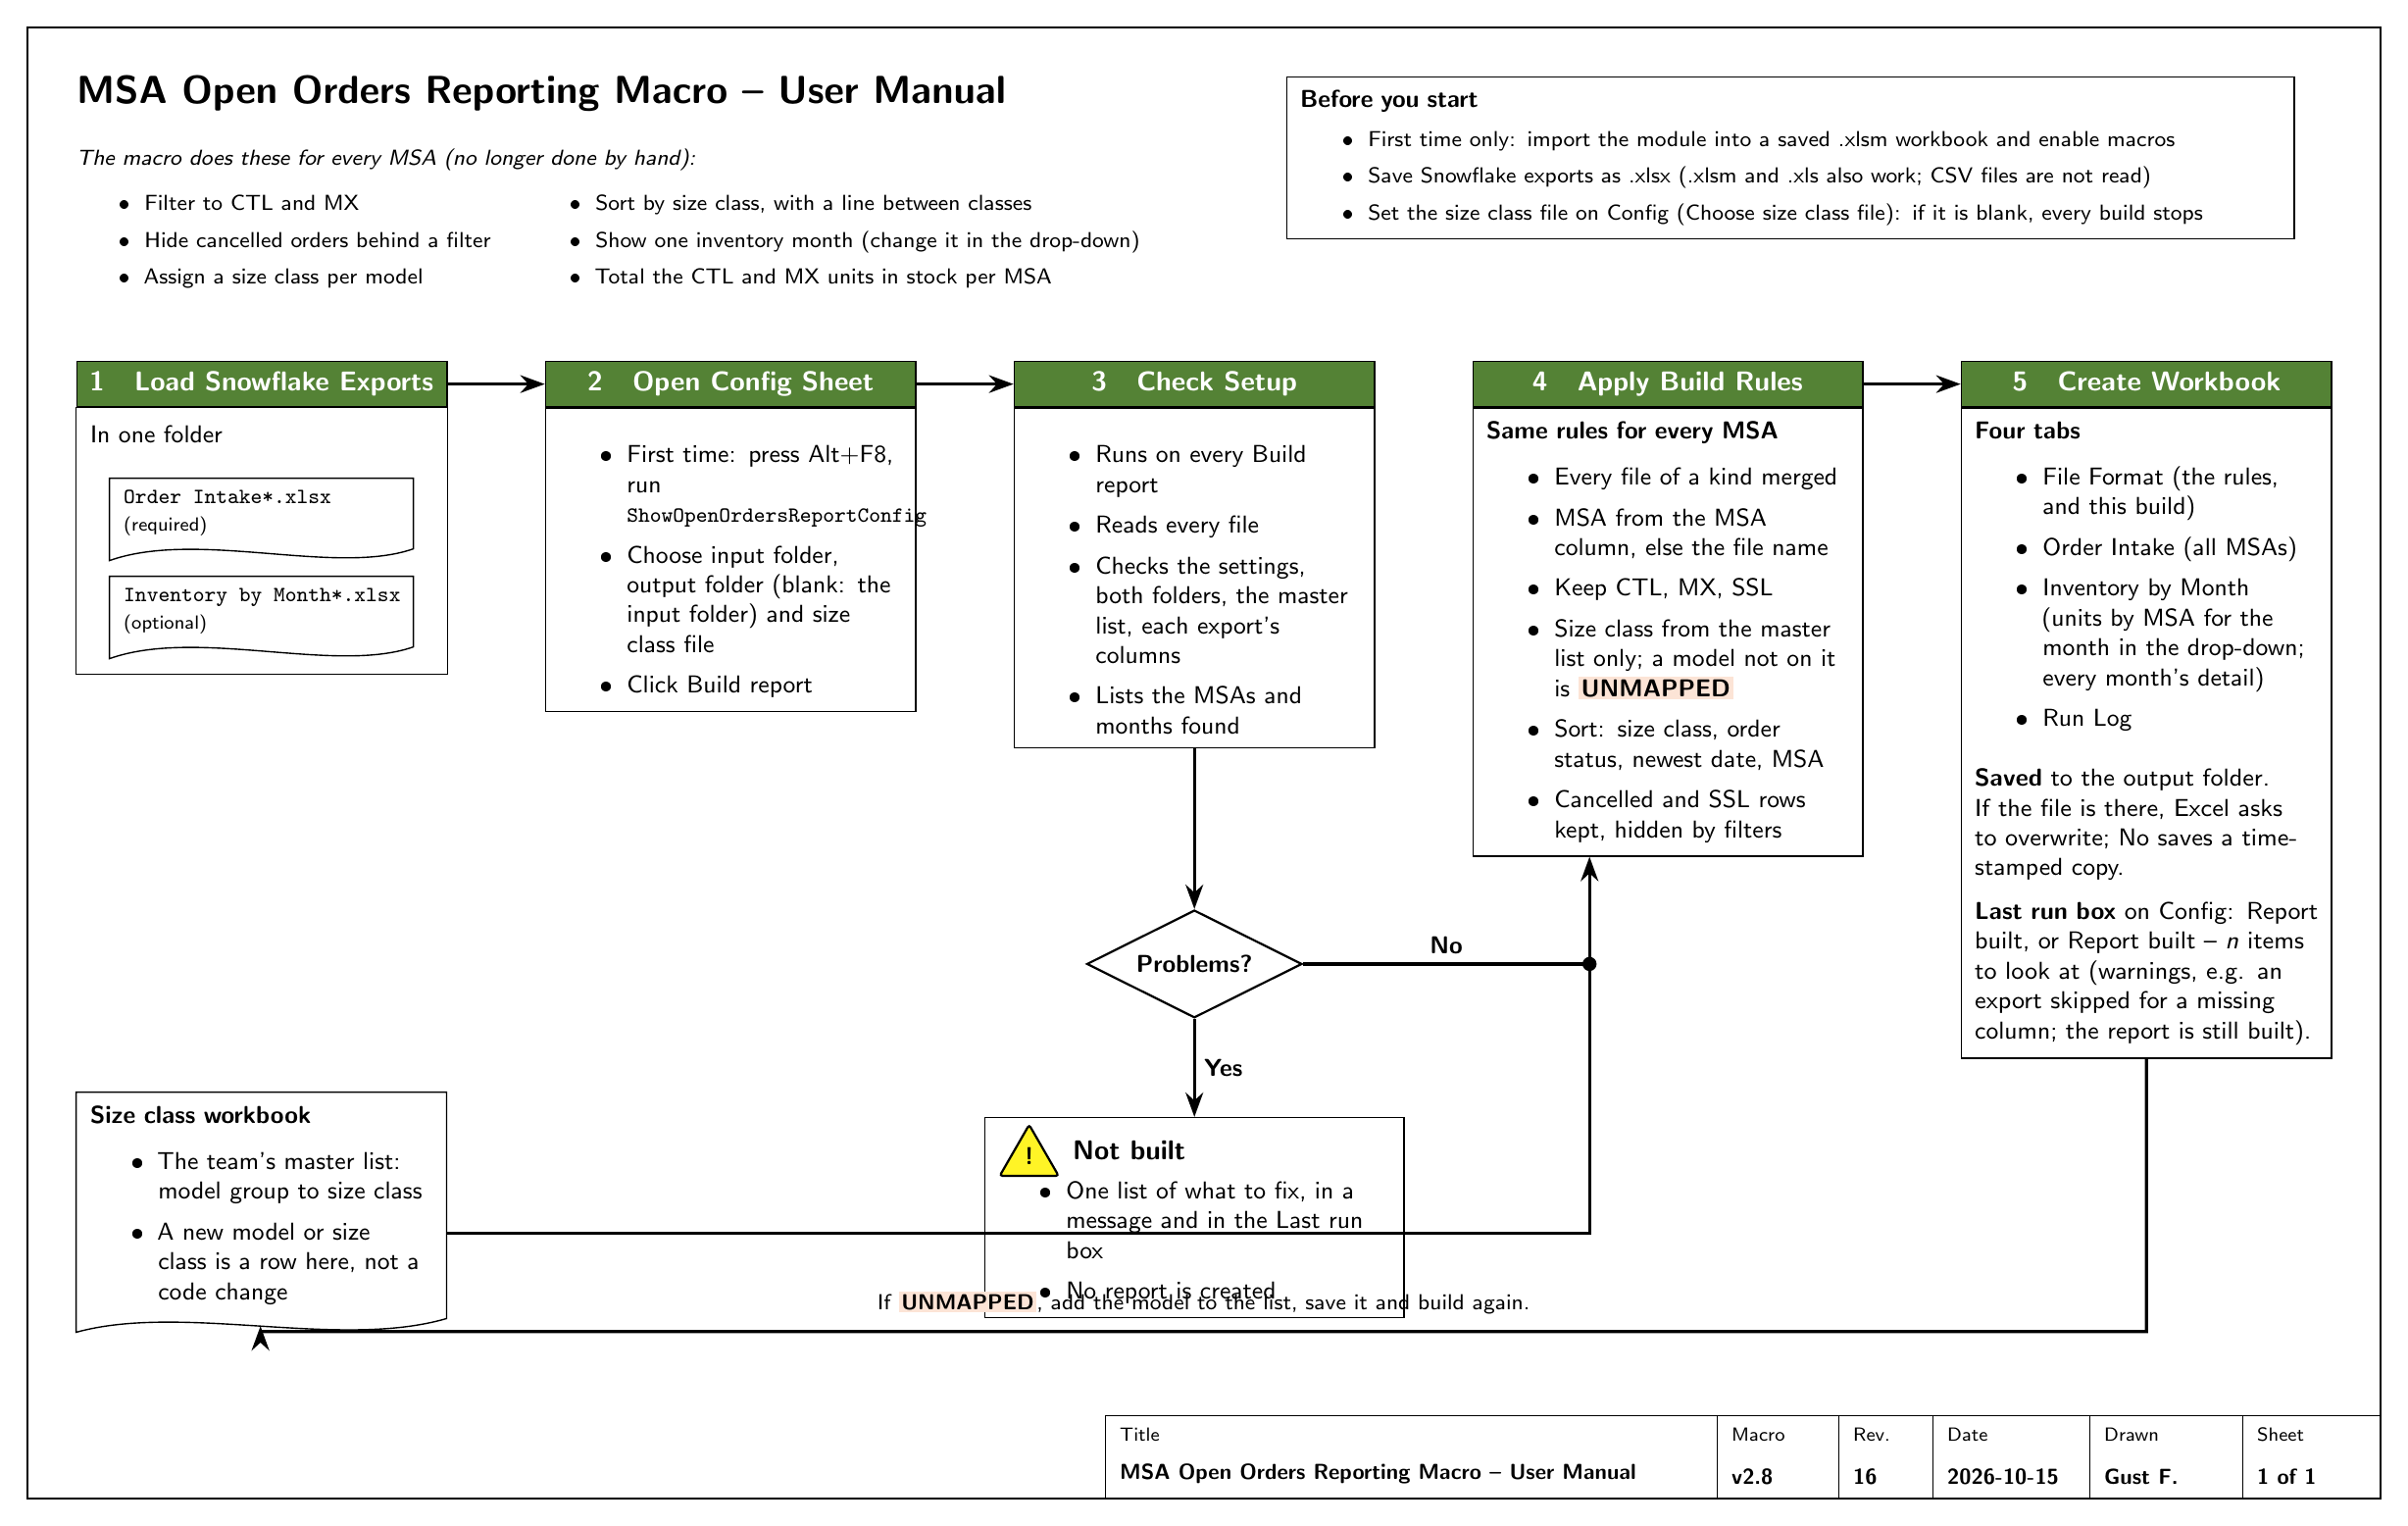
\begin{tikzpicture}[x=1in, y=1in]
\useasboundingbox (0,0) rectangle (12,7.5);

% ---------------------------------------------------------------- sheet frame
\draw[line width=0.8pt] (0,0) rectangle (12,7.5);

% ---------------------------------------------------------------- title and the by-hand line
\node[anchor=north west, inner sep=0pt, font=\sffamily\bfseries\fontsize{14}{16}\selectfont]
  at (0.25,7.25) {MSA Open Orders Reporting Macro -- User Manual};
\node[anchor=north west, inner sep=0pt, font=\sffamily\footnotesize\itshape] at (0.25,6.88) {The macro does these for every MSA (no longer done by hand):};
\node[anchor=north west, align=left, inner sep=0pt, text width=2.5in, font=\sffamily\footnotesize] at (0.25,6.74)
  {\begin{itemize}
  \item Filter to CTL and MX
  \item Hide cancelled orders behind a filter
  \item Assign a size class per model
  \end{itemize}};
\node[anchor=north west, align=left, inner sep=0pt, text width=3.3in, font=\sffamily\footnotesize] at (2.55,6.74)
  {\begin{itemize}
  \item Sort by size class, with a line between classes
  \item Show one inventory month (change it in the drop-down)
  \item Total the CTL and MX units in stock per MSA
  \end{itemize}};

% ---------------------------------------------------------------- before you start, top right
\node[box, anchor=north west, text width=5.0in, font=\sffamily\footnotesize] at (6.42,7.25) {\textbf{\small Before you start}\\[2pt]
  \begin{itemize}
  \item First time only: import the module into a saved .xlsm workbook and enable macros
  \item Save Snowflake exports as .xlsx (.xlsm and .xls also work; CSV files are not read)
  \item Set the size class file on Config (Choose size class file): if it is blank, every build stops
  \end{itemize}};

% ---------------------------------------------------------------- station 1: Snowflake exports, in one folder
\node[station, anchor=north west, text width=1.75in] (h1) at (0.25,5.8) {1\quad Load Snowflake Exports};
\draw[line width=0.5pt] (h1.south west) rectangle ($(h1.south east)+(0,-1.36)$);
\coordinate (b1) at ($(h1.south)+(0,-1.36)$);
\node[anchor=north west] at ($(h1.south west)+(0,-0.02)$) {In one folder};
\pic at ($(h1.south west)+(0.17,-0.36)$) {doc};
\node[anchor=north west, align=left, inner sep=0pt] at ($(h1.south west)+(0.24,-0.42)$)
  {{\footnotesize\texttt{Order Intake*.xlsx}}\\[-1pt]{\fontsize{7.5}{9}\selectfont(required)}};
\pic at ($(h1.south west)+(0.17,-0.86)$) {doc};
\node[anchor=north west, align=left, inner sep=0pt] at ($(h1.south west)+(0.24,-0.92)$)
  {{\footnotesize\texttt{Inventory by Month*.xlsx}}\\[-1pt]{\fontsize{7.5}{9}\selectfont(optional)}};

% ---------------------------------------------------------------- station 2: Config sheet
\node[station, anchor=north west, text width=1.75in] (h2) at (2.64,5.8) {2\quad Open Config Sheet};
\node[box, anchor=north, text width=1.75in] (b2) at (h2.south) {\begin{itemize}
  \item First time: press Alt+F8, run\\ {\footnotesize\texttt{ShowOpenOrdersReportConfig}}
  \item Choose input folder, output folder (blank: the input folder) and size class file
  \item Click Build report
  \end{itemize}};

% ---------------------------------------------------------------- station 3: setup check, the gate and the stop
\node[station, anchor=north west, text width=1.7in] (h3) at (5.03,5.8) {3\quad Check Setup};
\node[box, anchor=north, text width=1.7in] (b3) at (h3.south) {\begin{itemize}
  \item Runs on every Build report
  \item Reads every file
  \item Checks the settings, both folders, the master list, each export's columns
  \item Lists the MSAs and months found
  \end{itemize}};
\node[gate] (g) at ($(b3.south)+(0,-1.1)$) {Problems?};
\draw[flow] (b3.south) -- (g.north);
\node[box, anchor=north, text width=2.0in] (nb) at ($(g.south)+(0,-0.5)$) {{\normalsize\textbf{\phantom{Not built}}}\\[7pt]
  \begin{itemize}
  \item One list of what to fix, in a message and in the Last run box
  \item No report is created
  \end{itemize}};
\draw[flow] (g.south) -- (nb.north) node[midway, right, branch] {Yes};
% warning sign on the Not built box: the problem state (same sign as the manual's warning box)
\draw[line width=0.8pt, fill=yellow!85, rounded corners=1pt]
  ($(nb.north west)+(0.08,-0.3)$) -- ++(0.3,0) -- ++(-0.15,0.26) -- cycle;
\node[font=\sffamily\bfseries\small, inner sep=0pt] at ($(nb.north west)+(0.23,-0.2)$) {!};
\node[anchor=mid west, font=\sffamily\bfseries\normalsize, inner sep=0pt] at ($(nb.north west)+(0.45,-0.19)$) {Not built};

% ---------------------------------------------------------------- station 4: build
\node[station, anchor=north west, text width=1.85in] (h4) at (7.37,5.8) {4\quad Apply Build Rules};
\node[box, anchor=north, text width=1.85in] (b4) at (h4.south) {\textbf{Same rules for every MSA}\\[2pt]
  \begin{itemize}
  \item Every file of a kind merged
  \item MSA from the MSA column, else the file name
  \item Keep CTL, MX, SSL
  \item Size class from the master list only; a model not on it is {\setlength{\fboxsep}{1pt}\colorbox{flagpeach}{\textbf{UNMAPPED}}}
  \item Sort: size class, order status, newest date, MSA
  \item Cancelled and SSL rows kept, hidden by filters
  \end{itemize}};
% No: straight out of the gate until it joins the master-list line, which carries both up into Build
\coordinate (join) at ($(b4.south)+(-0.4,0)$);
\draw[line width=1.2pt] (g.east) -- (g.east -| join) node[pos=0.5, above, branch] {No};
\fill (g.east -| join) circle (2.6pt);

% ---------------------------------------------------------------- station 5: workbook
\node[station, anchor=north west, text width=1.75in] (h5) at (9.86,5.8) {5\quad Create Workbook};
\node[box, anchor=north, text width=1.75in] (b5) at (h5.south) {\textbf{Four tabs}\\[2pt]
  \begin{itemize}
  \item File Format (the rules, and this build)
  \item Order Intake (all MSAs)
  \item Inventory by Month (units by MSA for the month in the drop-down; every month's detail)
  \item Run Log
  \end{itemize}\vspace{5pt}
  \textbf{Saved} to the output folder. If the file is there, Excel asks to overwrite; No saves a time-stamped copy.\\[5pt]
  \textbf{Last run box} on Config: Report built, or Report built -- \textit{n} items to look at (warnings, e.g. an export skipped for a missing column; the report is still built).};

% ---------------------------------------------------------------- flow arrows along the header line
\draw[flow] (h1.east) -- (h2.west);
\draw[flow] (h2.east) -- (h3.west);
\draw[flow] (h4.east) -- (h5.west);

% ---------------------------------------------------------------- size class workbook, a document under station 1
\node[anchor=north west, align=left, text width=1.7in] (t6) at (0.25,2.07) {\textbf{Size class workbook}\\[2pt]
  \begin{itemize}
  \item The team's master list: model group to size class
  \item A new model or size class is a row here, not a code change
  \end{itemize}};
\draw[name path=scdoc, line width=0.5pt] (0.25,2.07) -- (2.139,2.07) -- (2.139,2.07 |- t6.south)
  .. controls ($(t6.south)+(0.42,-0.16)$) and ($(t6.south)+(-0.38,0.08)$) .. ($(0.25,0)+(0,0 |- t6.south)+(0,-0.07)$)
  -- cycle;

% master list into station 4: straight out of the document, one corner, up into Build
\draw[flow] (2.139,1.35) -| (join);

% return: UNMAPPED back to the master list, two right angles, ending on the document's wavy foot
\path[name path=up] (1.19,0) -- (1.19,2.07);
\path[name intersections={of=up and scdoc, sort by=up, by={foot}}];
\draw[flow] (b5.south) |- (1.19,0.85) -- (foot);
\node[anchor=south, note] at (6.0,0.91) {If {\setlength{\fboxsep}{1pt}\colorbox{flagpeach}{\textbf{UNMAPPED}}}, add the model to the list, save it and build again.};

% ---------------------------------------------------------------- title block, one row in the corner
\draw[line width=0.5pt] (5.5,0) -- (5.5,0.42) -- (12,0.42);
\foreach \x in {8.62, 9.24, 9.72, 10.52, 11.3} \draw[line width=0.5pt] (\x,0) -- (\x,0.42);
\foreach \x/\label/\value in {5.5/Title/MSA Open Orders Reporting Macro -- User Manual, 8.62/Macro/v2.8, 9.24/Rev./16,
                              9.72/Date/2026-10-15, 10.52/Drawn/Gust F., 11.3/Sheet/\flowsheet} {
  \node[anchor=north west, inner sep=0pt, font=\sffamily\fontsize{7}{8}\selectfont] at (\x+0.07,0.36) {\label};
  \node[anchor=south west, inner sep=0pt, font=\sffamily\bfseries\footnotesize] at (\x+0.07,0.07) {\value};
}

\end{tikzpicture}}
\end{document}
